\documentclass[11pt,a4paper]{article}

% =========================================================
% Single Bell Nozzle Geometry and Analysis Simulator
% Reorganized LaTeX manuscript
% =========================================================

% --- Page setup ---
\usepackage[a4paper,margin=22mm]{geometry}
\usepackage[utf8]{inputenc}
\usepackage[T1]{fontenc}
\usepackage{newtxtext,newtxmath}
\usepackage{microtype}
\usepackage{setspace}
\usepackage{indentfirst}
\usepackage{ragged2e}
\justifying

% --- Mathematics and units ---
\usepackage{amsmath,bm}
\usepackage{siunitx}
\sisetup{per-mode=symbol,detect-all=true}

% --- Figures and tables ---
\usepackage{graphicx}
\usepackage{float}
\usepackage{subcaption}
\usepackage{caption}
\usepackage{booktabs}
\usepackage{tabularx}
\usepackage{array}
\usepackage{adjustbox}
\usepackage{xcolor}
\usepackage{multicol}
\usepackage{enumitem}

% --- TikZ and plots ---
\usepackage{tikz}
\usepackage{pgfplots}
\pgfplotsset{compat=1.18}
\usetikzlibrary{calc,arrows.meta,angles,quotes,positioning}

% --- Headers, links and bibliography ---
\usepackage{fancyhdr}
\usepackage{lastpage}
\usepackage[hidelinks]{hyperref}

% --- Compact paragraph/list formatting ---
\setlength{\parskip}{4pt}
\setlength{\parindent}{12pt}
\setlist[itemize]{topsep=3pt,itemsep=2pt,parsep=0pt}
\setlist[enumerate]{topsep=3pt,itemsep=2pt,parsep=0pt}
\setcounter{tocdepth}{2} % show sections and broad subsections only; subsubsections stay out of the table of contents
\setcounter{secnumdepth}{3}

% --- Header logo fallback: works whether the logo is in root or Images/ ---
\newcommand{\PSTlogo}{%
\IfFileExists{Images/invictus-1c9f019a.png}{
\includegraphics[height=8mm]{Images/invictus-1c9f019a.png}}{%
\IfFileExists{invictus-1c9f019a.png}{
\includegraphics[height=8mm]{invictus-1c9f019a.png}}{}}}

\setlength{\headheight}{14pt}
\pagestyle{fancy}
\fancyhf{}
\lhead{\PSTlogo}
\rhead{\nouppercase{\leftmark}}
\lfoot{Single Bell Nozzle Geometry and Analysis Simulator}
\rfoot{\thepage/\pageref{LastPage}}
\renewcommand{\headrulewidth}{0.4pt}
\renewcommand{\footrulewidth}{0.4pt}

\title{\textbf{Single Bell Nozzle Geometry and Analysis Simulator}}
\author{
Rafael Lino$^{1,2}$\\
\small $^1$Porto Space Team, Faculty of Engineering, University of Porto, Porto, Portugal\\
\small $^2$Department of Mechanical Engineering, Faculty of Engineering, University of Porto, Porto, Portugal
}
\date{April 2025}

\begin{document}

% =========================================================
% COVER
% =========================================================
\begin{titlepage}
\thispagestyle{empty}

\begin{minipage}[t]{0.45\linewidth}
\PSTlogo
\end{minipage}
\hfill
\begin{minipage}[t]{0.5\linewidth}
\raggedleft
{\large \textbf{INVICTUS Project -- Propulsion Department}}\\[2pt]
\normalsize Faculty of Engineering, University of Porto
\end{minipage}

\vspace{22mm}

{\LARGE\bfseries Single Bell Nozzle Geometry and Analysis Simulator\par}
\vspace{3mm}
\hrule height 0.7pt
\vspace{4mm}
{\large Geometric formulation, isentropic flow analysis, 3D generation, CAD export, and genetic optimization framework\par}

\vspace{14mm}

\renewcommand{\arraystretch}{1.25}
\begin{tabularx}{\linewidth}{@{}>{\bfseries}l X@{}}
\toprule
Author & Rafael Lino \\
Project & INVICTUS / Porto Space Team \\
Document type & Reorganized technical article draft \\
Main topic & Single bell nozzle geometry and preliminary performance analysis \\
Future extension & Genetic algorithm optimization with geometric and viscous losses \\
\bottomrule
\end{tabularx}

\vspace{14mm}

\noindent\textbf{Abstract}\\[2pt]
This work presents the formulation and development of a computational simulator for the geometric generation and preliminary analysis of single bell nozzles for hybrid rocket propulsion systems. The simulator supports fast nozzle sizing, two-dimensional contour generation, three-dimensional visualization, coordinate export to CAD software, and preliminary performance estimation based on thermochemical data and quasi-one-dimensional nozzle relations.

The nozzle contour follows a classical bell geometry inspired by the Rao--Sutton approach, combining a converging subsonic section, a rounded throat region, a short supersonic circular arc, and a parabolic diverging contour. The main geometric design variables are the throat radius, expansion ratio, chamber radius, converging angle, initial supersonic angle, reference conical half-angle, and bell length fraction. From these variables, the simulator constructs a continuous piecewise contour and evaluates secondary geometric quantities such as contraction ratio, nozzle length, exit radius, and parabolic exit angle.

The baseline flow model assumes steady, adiabatic, quasi-one-dimensional, inviscid, shock-free expansion. Thermochemical properties are obtained from NASA CEA through RocketCEA, while the axial Mach-number, static-pressure and static-temperature distributions are reconstructed station-by-station from the generated area distribution, the area--Mach relation and the classical isentropic relations. This ideal framework is later extended with simplified geometric and viscous loss models suitable for integration into a genetic optimization algorithm, including exit divergence losses, boundary-layer blockage effects, and curvature-based turning penalties.

\vfill
\noindent\textbf{Keywords:} bell nozzle; hybrid rocket engine; nozzle geometry; isentropic flow; RocketCEA; boundary layer; genetic algorithm; propulsion optimization.

\vspace{6mm}
\hrule height 0.7pt
\vspace{2mm}
\small Internal draft -- Porto Space Team. Page 1 of \pageref{LastPage}.

\end{titlepage}

\newpage
\tableofcontents
\newpage
\listoffigures
\newpage

% =========================================================
\section{Introduction}
% =========================================================

Rocket nozzle geometry is one of the dominant factors controlling the conversion of chamber thermal energy into directed exhaust kinetic energy. For a fixed chamber pressure, propellant mass flow rate and propellant combination, the nozzle determines the exhaust Mach number, exit pressure, exit velocity, thrust coefficient and degree of axial momentum alignment. An efficient nozzle must therefore expand the combustion gases as much as possible while avoiding excessive length, excessive divergence losses, flow separation, shock formation or manufacturing complexity.

Among the most common rocket nozzle configurations, the bell nozzle offers a strong compromise between performance and compactness. A purely conical nozzle is simple to manufacture and analyze, but its constant wall angle produces larger divergence losses for a given length. A bell nozzle replaces most of the conical diverging section with a curved contour, allowing strong initial expansion immediately downstream of the throat and a smaller exit angle at the nozzle exit. This improves axial momentum alignment while maintaining a shorter nozzle than an equivalent low-angle conical design.

The simulator described in this work was created to generate and analyze single bell nozzle geometries for hybrid rocket engines, with emphasis on a paraffin wax and nitrous oxide propulsion system. The original work mixed implementation details, code excerpts, theoretical derivations, geometry construction and results in the same sections. This revised manuscript separates the material into four layers: physical theory, geometric formulation, numerical implementation logic, and results/optimization interpretation.

The simulator is intended as a preliminary engineering tool rather than a final qualification model. Its value lies in the explicit connection between geometry, ideal flow relations, visualization, CAD export and performance trends. The structure presented here also prepares the model for later integration with a genetic algorithm, where geometric parameters can be optimized automatically.


% =========================================================
\section{Objectives and Scope}
% =========================================================

The simulator has two main purposes. The first is to provide a fast preliminary design tool for a single bell nozzle, from basic propulsion inputs to a usable geometric contour. The second is to create a mathematical framework in which nozzle geometry can later be optimized automatically, particularly through a genetic algorithm.

The present formulation focuses on:
\begin{enumerate}
    \item geometric definition of a single bell nozzle contour;
    \item calculation of throat radius from ideal choked-flow relations;
    \item calculation of exit radius from a prescribed expansion ratio;
    \item estimation of an ideal expansion ratio for a chosen operating altitude or ambient pressure;
    \item computation of ideal isentropic flow properties along the nozzle;
    \item three-dimensional visualization by revolution of the two-dimensional contour;
    \item coordinate export for CAD modeling and manufacturing preparation;
    \item definition of geometric and viscous efficiency factors for future optimization.
\end{enumerate}

The simulator is not intended to replace detailed CFD, method-of-characteristics nozzle design, finite-rate chemistry, structural analysis, thermal analysis or experimental validation. Instead, it provides a fast, interpretable and modifiable preliminary model. Its strongest value is not absolute prediction accuracy, but the ability to connect geometric parameters to performance trends in a controlled and computationally inexpensive way.

% =========================================================
\section{Baseline Quasi-One-Dimensional Inviscid Nozzle Flow Model}
% =========================================================

\subsection{Thermodynamic closure and governing relations}

\subsubsection{Governing assumptions}

The baseline analysis is based on the classical quasi-one-dimensional nozzle model. The following assumptions are used in the ideal formulation:
\begin{itemize}
    \item the flow is steady;
    \item the flow is adiabatic;
    \item the flow is inviscid in the core region;
    \item the nozzle flow is shock-free;
    \item the gas expansion is treated as isentropic;
    \item the flow is quasi-one-dimensional, meaning that properties vary mainly along the nozzle axis;
    \item the gas is approximated as a perfect gas with an effective specific heat ratio $\gamma$;
    \item sonic conditions occur at the throat for a choked nozzle;
    \item the throat area is equal to the critical area, $A_t=A^*$;
    \item the subsonic branch of the area--Mach relation is used upstream of the throat;
    \item the supersonic branch is used downstream of the throat.
\end{itemize}

These assumptions are appropriate for preliminary design. They are not sufficient for final qualification of a rocket nozzle because they neglect real-gas effects, finite-rate chemistry, wall heat transfer, boundary-layer separation, shocks, nonuniform inlet conditions, two-phase particles or droplets, and multidimensional wave structures.

\subsubsection{Thermochemical closure using NASA CEA/RocketCEA}

The thermochemical properties used by the simulator are obtained from NASA CEA through RocketCEA. For each combination of chamber pressure, mixture ratio and expansion ratio, RocketCEA can provide useful quantities such as combustion temperature, effective ratio of specific heats, molar mass of combustion products, characteristic velocity, thrust coefficient, exit Mach number, exit temperature, exit pressure and ideal specific impulse.

In the simplest model, $\gamma$ is treated as constant along the nozzle. This is a simplification, because the chemical composition and thermodynamic properties of the combustion products may vary during expansion. However, the constant-$\gamma$ approximation is useful for deriving closed-form relations and for keeping the simulator fast and transparent.

For a hybrid engine using nitrous oxide and paraffin-based fuel, RocketCEA also allows the user to define a custom fuel composition and evaluate equilibrium combustion properties for the chosen oxidizer-to-fuel ratio.

\subsubsection{Choked mass-flow constraint and throat sizing}

For a choked nozzle, the mass flow rate through the throat is governed by the stagnation conditions upstream of the throat and by the throat area. Assuming isentropic perfect-gas flow, the choked mass flow rate is
\begin{equation}
\dot{m}=A_t P_0
\sqrt{\frac{\gamma}{R T_0}}
\left(\frac{2}{\gamma+1}\right)^{\frac{\gamma+1}{2(\gamma-1)}} .
\label{eq:choked_mdot}
\end{equation}

Solving for throat area gives
\begin{equation}
A_t =
\frac{\dot{m}}{P_0
\sqrt{\dfrac{\gamma}{R T_0}}
\left(\dfrac{2}{\gamma+1}\right)^{\frac{\gamma+1}{2(\gamma-1)}}} ,
\label{eq:throat_area}
\end{equation}
with
\begin{equation}
r_t=\sqrt{\frac{A_t}{\pi}} .
\label{eq:throat_radius}
\end{equation}

This relation links the propulsion operating point to the geometry. For a fixed chamber pressure and combustion temperature, increasing mass flow requires a larger throat area. For a fixed mass flow rate, increasing chamber pressure allows the same mass flow through a smaller throat.

\begin{figure}[H]
    \centering
    \IfFileExists{cad5.png}{
\includegraphics[width=0.75\linewidth]{cad5.png}}{\fbox{\parbox{0.75\linewidth}{\centering Missing figure file: \texttt{cad5.png}}}}
    \caption{Nozzle flow stations used for throat sizing and ideal one-dimensional analysis.}
    \label{fig:flow_stations}
\end{figure}

\subsubsection{Thrust balance and ideal expansion criterion}

The thrust produced by a rocket nozzle can be approximated by
\begin{equation}
F=\dot{m}V_e+(p_e-p_a)A_e,
\label{eq:thrust}
\end{equation}
where $V_e$ is the exit velocity, $p_e$ is the nozzle exit pressure, $p_a$ is the ambient pressure and $A_e$ is the exit area.

The first term is the momentum thrust. The second term is the pressure thrust. For a fixed chamber condition and mass flow rate, the ideal expansion condition at a given altitude is approximately
\begin{equation}
p_e=p_a .
\label{eq:ideal_expansion}
\end{equation}

When $p_e>p_a$, the nozzle is underexpanded and the gases still have remaining expansion potential at the exit. When $p_e<p_a$, the nozzle is overexpanded, which can lead to compression waves, shocks, separation risk and loss of performance depending on the operating regime.

Because ambient pressure varies during flight, a fixed-geometry nozzle cannot be perfectly expanded at all altitudes. For low-altitude or short-duration flights, the simulator may use a representative ambient pressure, such as sea-level pressure or a trajectory-averaged ambient pressure. For a more complete flight analysis, the expansion ratio should be evaluated over the expected altitude range and the selected value should minimize a trajectory-weighted performance penalty.

\subsubsection{Expansion ratio and exit-plane radius}

The expansion ratio is defined as
\begin{equation}
\varepsilon=\frac{A_e}{A_t} .
\label{eq:expansion_ratio}
\end{equation}

For circular sections,
\begin{equation}
\varepsilon=\frac{\pi r_e^2}{\pi r_t^2}=\left(\frac{r_e}{r_t}\right)^2,
\end{equation}
therefore
\begin{equation}
r_e=\sqrt{\varepsilon}\,r_t .
\label{eq:exit_radius}
\end{equation}

The expansion ratio is one of the most important nozzle design variables. Increasing $\varepsilon$ generally increases exit Mach number and ideal exhaust velocity, but also increases nozzle length, exit area, structural mass and overexpansion risk at low altitude.

\subsubsection{Propellant mass-flow closure from mixture ratio}

Using the conventional definition
\begin{equation}
O/F=\frac{\dot{m}_{ox}}{\dot{m}_{fuel}},
\end{equation}
the fuel mass flow rate is
\begin{equation}
\dot{m}_{fuel}=\frac{\dot{m}_{ox}}{O/F},
\end{equation}
and the total propellant mass flow rate is
\begin{equation}
\dot{m}_{prop}=\dot{m}_{ox}+\dot{m}_{fuel}
=\dot{m}_{ox}\left(1+\frac{1}{O/F}\right).
\label{eq:mdot_total}
\end{equation}

This convention must be used consistently. Reversing the definition of mixture ratio changes the mass-flow calculation and therefore the throat sizing.

% 
% =========================================================

\subsection{Axial flow-field reconstruction}

\subsubsection{Stagnation-to-static isentropic relations}

For one-dimensional, steady, adiabatic and inviscid flow of a perfect gas, the stagnation-to-static relations are
\begin{align}
\frac{T}{T_0} &= \left(1+\frac{\gamma-1}{2}M^2\right)^{-1},
\label{eq:T_T0}\\
\frac{p}{p_0} &= \left(1+\frac{\gamma-1}{2}M^2\right)^{-\gamma/(\gamma-1)},
\label{eq:p_p0}\\
\frac{\rho}{\rho_0} &= \left(1+\frac{\gamma-1}{2}M^2\right)^{-1/(\gamma-1)}.
\label{eq:rho_rho0}
\end{align}

Once the Mach number distribution $M(x)$ is known, these relations provide the axial distributions of temperature, pressure and density.

\subsubsection{Area--Mach compatibility relation}

The Mach number is implicitly related to the local cross-sectional area through the area--Mach relation:
\begin{equation}
\frac{A}{A^*}=\frac{1}{M}
\left[
\frac{2}{\gamma+1}
\left(1+\frac{\gamma-1}{2}M^2\right)
\right]^{\frac{\gamma+1}{2(\gamma-1)}} .
\label{eq:area_mach}
\end{equation}

For a choked nozzle, $A^*=A_t$. Therefore, at each axial station,
\begin{equation}
\frac{A(x)}{A_t}=\frac{\pi r(x)^2}{\pi r_t^2}=\left(\frac{r(x)}{r_t}\right)^2 .
\label{eq:area_ratio_local}
\end{equation}

Equation~\eqref{eq:area_mach} has two possible Mach solutions for $A/A^*>1$: a subsonic solution and a supersonic solution. The correct branch is selected from the location relative to the throat. Upstream of the throat, the subsonic solution is used. Downstream of the throat, the supersonic solution is used. At the throat, $M=1$.

\subsubsection{Branch-resolved numerical solution of the Mach number}

Because Eq.~\eqref{eq:area_mach} cannot generally be inverted explicitly for $M$, the simulator determines $M(x)$ by solving
\begin{equation}
f(M)=\frac{A}{A^*} - \frac{1}{M}
\left[
\frac{2}{\gamma+1}
\left(1+\frac{\gamma-1}{2}M^2\right)
\right]^{\frac{\gamma+1}{2(\gamma-1)}}=0 .
\label{eq:area_mach_residual}
\end{equation}

Two robust numerical strategies are suitable:
\begin{itemize}
    \item \textbf{bisection}, which is slower but stable if the bracket contains a root;
    \item \textbf{Newton--Raphson}, which is faster but requires a good initial guess.
\end{itemize}

For a preliminary simulator, bisection is often preferable because it avoids convergence failures near the throat or when the first estimate is poor. The usual numerical intervals are
\begin{equation}
M\in(0,1) \quad \text{for the subsonic branch},
\end{equation}
\begin{equation}
M\in(1,M_{max}) \quad \text{for the supersonic branch}.
\end{equation}

Once $M(x)$ is obtained, the local speed of sound and axial velocity are
\begin{equation}
a(x)=\sqrt{\gamma R T(x)},
\end{equation}
\begin{equation}
u(x)=M(x)a(x).
\label{eq:velocity}
\end{equation}


\subsubsection{Axial reconstruction of Mach, static-pressure and static-temperature curves}

The axial property curves are obtained by coupling the piecewise radius function to the quasi-one-dimensional isentropic model. The process starts from the discretized nozzle contour,
\begin{equation}
\left\{x_i,r_i\right\}_{i=0}^{N},
\end{equation}
where each station has the local cross-sectional area
\begin{equation}
A_i=\pi r_i^2.
\label{eq:local_area_discrete}
\end{equation}

Because the throat is assumed choked, the critical area is
\begin{equation}
A^*=A_t=\pi r_t^2.
\end{equation}
Therefore, the local area ratio used in the area--Mach equation is
\begin{equation}
\Lambda_i=\frac{A_i}{A_t}=\left(\frac{r_i}{r_t}\right)^2.
\label{eq:local_area_ratio_discrete}
\end{equation}

For each station, the Mach number is obtained by solving the residual form of the area--Mach equation,
\begin{equation}
F(M_i,\Lambda_i)=
\frac{1}{M_i}
\left[
\frac{2}{\gamma+1}
\left(1+\frac{\gamma-1}{2}M_i^2\right)
\right]^{\frac{\gamma+1}{2(\gamma-1)}}
-\Lambda_i=0.
\label{eq:mach_curve_residual}
\end{equation}

The solution branch is selected from the geometric station location:
\begin{equation}
0<M_i<1 \quad \text{for} \quad x_i<x_t,
\end{equation}
\begin{equation}
M_i=1 \quad \text{for} \quad x_i=x_t,
\end{equation}
\begin{equation}
M_i>1 \quad \text{for} \quad x_i>x_t.
\end{equation}
This branch selection is essential because the area--Mach relation is double-valued for \(A/A^*>1\). The same area ratio may correspond either to a subsonic state upstream of the throat or to a supersonic state downstream of it.

After the Mach number has been obtained at each station, the static-temperature curve is generated directly from the stagnation-to-static relation,
\begin{equation}
T_i=T(x_i)=\frac{T_0}{1+\dfrac{\gamma-1}{2}M_i^2}.
\label{eq:temperature_curve}
\end{equation}
Similarly, the static-pressure curve is obtained from
\begin{equation}
p_i=p(x_i)=p_0
\left(1+\frac{\gamma-1}{2}M_i^2\right)^{-\gamma/(\gamma-1)}.
\label{eq:pressure_curve}
\end{equation}
The density curve may also be reconstructed as
\begin{equation}
\rho_i=\rho(x_i)=\rho_0
\left(1+\frac{\gamma-1}{2}M_i^2\right)^{-1/(\gamma-1)}.
\label{eq:density_curve}
\end{equation}

The simulator therefore stores the axial flow-field dataset as
\begin{equation}
\mathcal{D}_{flow}=\left\{x_i,\,A_i,\,\Lambda_i,\,M_i,\,T_i,\,p_i,\,\rho_i,\,u_i\right\}_{i=0}^{N},
\label{eq:flow_dataset}
\end{equation}
where the velocity is obtained from
\begin{equation}
u_i=M_i\sqrt{\gamma R T_i}.
\label{eq:velocity_curve}
\end{equation}

The Mach, pressure and temperature curves are then plotted as functions of the translated axial coordinate \(\bar{x}\). This means that the plotted distributions are not read directly from CEA along the nozzle. CEA/RocketCEA provides the thermochemical closure and reference stagnation properties, while the spatial evolution along the generated contour is reconstructed from \(r(x)\), the area--Mach relation and the isentropic equations.

In the converging subsonic region, reducing area accelerates the flow and increases Mach number toward unity. At the throat, the nozzle becomes choked and $M=1$. In the diverging supersonic region, increasing area further accelerates the flow and produces a supersonic Mach number increase.

The temperature and pressure decrease throughout the expansion according to Eqs.~\eqref{eq:T_T0} and~\eqref{eq:p_p0}. Therefore, the simulator can generate axial distributions of Mach number, pressure and temperature from the geometric contour alone, once the chamber stagnation state and thermodynamic model have been selected.

\begin{figure}[H]
    \centering
    \IfFileExists{ex24.png}{
\includegraphics[width=0.82\linewidth]{ex24.png}}{\fbox{\parbox{0.82\linewidth}{\centering Missing figure file: \texttt{ex24.png} or replace with the Mach/pressure/temperature axial plot generated by the simulator.}}}
    \caption{Representative axial reconstruction of Mach number, static pressure and static temperature from the generated nozzle contour.}
    \label{fig:axial_mach_pressure_temperature}
\end{figure}

\newpage

% ==================================================================================================================
\section{Loss-Corrected Quasi-One-Dimensional Model for Geometry Optimization}
% =========================================================

\subsection{Reduced-order loss mechanisms}

\subsubsection{Need for loss-corrected optimization}

The ideal isentropic model is useful for generating trends, but a genetic algorithm can exploit weaknesses in an oversimplified model. For example, if only ideal exhaust velocity is maximized, the optimizer may choose geometries that are theoretically high-performing but physically poor: very short contours, excessive wall turning, large exit angles, unrealistic curvature or excessive boundary-layer blockage.

For this reason, the optimization model should not rely only on the ideal expansion equations. It should also include loss mechanisms that penalize geometries with poor physical behavior. The present formulation introduces three efficiency factors:
\begin{equation}
\eta_{total}=\eta_{div}\eta_{BL}\eta_{turn}.
\label{eq:eta_total_intro}
\end{equation}

These terms do not replace CFD or experimental calibration, but they provide a physically interpretable bridge between geometry and optimization.

\subsubsection{Exit-flow divergence loss model}

In an ideal nozzle, the exhaust flow would leave perfectly aligned with the nozzle axis. In a real finite-length nozzle, the exit flow has a radial component caused by the exit wall angle. Assuming that the exit flow angle is approximately equal to the local contour angle $\theta_{out}$, the axial momentum efficiency can be estimated by a geometric projection:
\begin{equation}
\boxed{\eta_{div}=\cos(\theta_{out})}.
\label{eq:eta_div}
\end{equation}

This term penalizes large exit angles. It also creates a natural trade-off: decreasing $\theta_{out}$ usually requires a longer nozzle or a different parabolic contour.

\subsubsection{Boundary-layer displacement and effective-area blockage}

As the hot gas expands through the nozzle, viscous effects become important near the wall. The no-slip condition imposes zero velocity at the wall, while the inviscid core flow remains faster away from the wall. The resulting boundary layer produces shear stress, entropy generation and an effective reduction of the flow area available to the inviscid core.

The displacement thickness $\delta^*(x)$ represents the virtual inward displacement of the wall that would produce the same mass-flow deficit in an inviscid equivalent flow. For turbulent flow over a smooth wall, a preliminary estimate is
\begin{equation}
\delta^*(x)=0.046\frac{x}{Re_x^{1/5}},
\label{eq:delta_star}
\end{equation}
where
\begin{equation}
Re_x=\frac{\rho(x)u(x)x}{\mu(x)}.
\label{eq:Rex}
\end{equation}

The effective radius is then
\begin{equation}
r_{eff}(x)=r(x)-\delta^*(x),
\label{eq:reff}
\end{equation}
and the effective area becomes
\begin{equation}
A_{eff}(x)=\pi r_{eff}^2(x).
\label{eq:Aeff}
\end{equation}

The Mach distribution can be recomputed using $A_{eff}(x)$ instead of the purely geometric area. This produces an effective exit velocity $V_{e,eff}$, which can be compared with the ideal isentropic value $V_{e,ist}$:
\begin{equation}
\boxed{\eta_{BL}=\frac{V_{e,eff}}{V_{e,ist}}}.
\label{eq:eta_BL}
\end{equation}

A more rigorous future version should also consider the displacement thickness at the throat and its effect on choking. The present model is suitable as a first penalty term for geometry optimization, not as a final viscous-flow solver.

\subsubsection{Curvature-based turning loss model}

The initial supersonic angle $\theta_{in}$ controls the rate at which the wall turns the flow immediately downstream of the throat. In supersonic flow, rapid turning over short axial distances can generate expansion and compression wave systems, local entropy production and additional viscous losses. These effects are not captured by exit divergence alone.

To include the shape of the contour, a curvature-based turning metric is introduced. For a planar contour $r(x)$, the curvature is
\begin{equation}
\kappa(x)=\frac{|r''(x)|}{\left[1+r'(x)^2\right]^{3/2}}.
\label{eq:curvature_general}
\end{equation}

For the parabolic section,
\begin{equation}
r(x)=ax^2+bx+c,
\end{equation}
so
\begin{equation}
r'(x)=2ax+b,
\end{equation}
\begin{equation}
r''(x)=2a,
\end{equation}
and therefore
\begin{equation}
\kappa(x)=\frac{|2a|}{\left[1+(2ax+b)^2\right]^{3/2}}.
\label{eq:curvature_parabola}
\end{equation}

The cumulative turning severity may be measured by integrating curvature along the arc length:
\begin{equation}
\Phi_s=\int_{x_P}^{L}\kappa(x)\sqrt{1+r'(x)^2}\,dx.
\label{eq:Phi_s}
\end{equation}

A turning efficiency can then be defined as
\begin{equation}
\boxed{\eta_{turn}=\exp(-k\Phi_s)},
\label{eq:eta_turn}
\end{equation}
where $k$ is an empirical calibration coefficient. This form guarantees $0<\eta_{turn}\leq1$ and penalizes geometries that concentrate strong curvature in the early supersonic region.

\newpage


\section{Expansion-Ratio Selection and Ideal Performance Mapping}
% =========================================================

\subsection{Ideal operating-point and performance maps}

\subsubsection{Ambient-pressure matching and expansion-ratio search}

For a given chamber pressure, mixture ratio and propellant combination, the simulator can estimate the expansion ratio that best matches the desired ambient pressure. The ideal criterion is
\begin{equation}
p_e(\varepsilon)=p_a.
\label{eq:epsilon_target}
\end{equation}

The numerical search evaluates the exit pressure for a range of expansion ratios and selects the value that minimizes
\begin{equation}
E_{\varepsilon}=\left|p_e(\varepsilon)-p_a\right|.
\label{eq:epsilon_error}
\end{equation}

If the search is performed for several chamber pressures, the result can be plotted as an ideal expansion-ratio curve. Interpolation may then be used to estimate an appropriate $\varepsilon$ for intermediate chamber pressures.

\begin{figure}[H]
    \centering
    \IfFileExists{ex19.png}{
\includegraphics[width=0.82\linewidth]{ex19.png}}{\fbox{\parbox{0.82\linewidth}{\centering Missing figure file: \texttt{ex19.png}}}}
    \caption{Example output for ideal expansion ratio estimation.}
    \label{fig:ideal_expansion_result}
\end{figure}

\subsubsection{Exit velocity and exit-temperature evaluation}

Under the ideal isentropic model, the exhaust velocity can be estimated from the chamber temperature and exit temperature:
\begin{equation}
V_e=\sqrt{\frac{2\gamma}{\gamma-1}RT_0\left[1-\left(\frac{p_e}{p_0}\right)^{(\gamma-1)/\gamma}\right]}.
\label{eq:ve_pressure}
\end{equation}

Equivalently, once the exit Mach number is known,
\begin{equation}
V_e=M_e\sqrt{\gamma R T_e}.
\label{eq:ve_mach}
\end{equation}

The exit temperature is obtained from Eq.~\eqref{eq:T_T0}:
\begin{equation}
T_e=\frac{T_0}{1+\dfrac{\gamma-1}{2}M_e^2}.
\label{eq:Te}
\end{equation}

The simulator can therefore plot exhaust velocity and exhaust temperature as functions of chamber pressure, expansion ratio or mixture ratio. These plots help identify the sensitivity of nozzle performance to the operating point.

\begin{figure}[H]
    \centering
    \begin{subfigure}{0.48\linewidth}
        \centering
        \IfFileExists{ex20.png}{
\includegraphics[width=\linewidth]{ex20.png}}{\fbox{\parbox{0.95\linewidth}{\centering Missing: \texttt{ex20.png}}}}
        \caption{Example exhaust velocity trend.}
    \end{subfigure}
    \hfill
    \begin{subfigure}{0.48\linewidth}
        \centering
        \IfFileExists{ex21.png}{
\includegraphics[width=\linewidth]{ex21.png}}{\fbox{\parbox{0.95\linewidth}{\centering Missing: \texttt{ex21.png}}}}
        \caption{Example exhaust temperature trend.}
    \end{subfigure}
    \caption{Example performance plots generated by the simulator.}
    \label{fig:exhaust_plots}
\end{figure}

\subsubsection{Thrust coefficient, characteristic velocity and specific impulse}

The main ideal performance parameters are:
\begin{align}
I_{sp} &= \frac{F}{\dot{m}g_0},
\label{eq:Isp}\\
c^* &= \frac{p_c A_t}{\dot{m}},
\label{eq:cstar}\\
C_F &= \frac{F}{p_c A_t}.
\label{eq:CF}
\end{align}

The characteristic velocity $c^*$ mainly measures combustion and thermochemical performance, while the thrust coefficient $C_F$ measures how effectively the nozzle converts chamber pressure into thrust. The specific impulse $I_{sp}$ combines the full propulsion performance into an impulse per unit propellant weight flow.

\begin{figure}[H]
    \centering
    \IfFileExists{ex23.png}{
\includegraphics[width=0.82\linewidth]{ex23.png}}{\fbox{\parbox{0.82\linewidth}{\centering Missing figure file: \texttt{ex23.png}}}}
    \caption{Example performance-parameter output table and plot.}
    \label{fig:performance_parameters}
\end{figure}

% 

\newpage
% =========================================================
\section{Parametric Rao--Sutton Bell-Nozzle Geometry Formulation}
% =========================================================

\subsection{Analytical contour definition}

\subsubsection{Independent geometric design parameters}

The nozzle geometry is defined by a reduced set of parameters:
\begin{itemize}
    \item throat radius, $r_t$;
    \item chamber radius, $r_c$;
    \item expansion ratio, $\varepsilon$;
    \item subsonic converging angle, $\theta_{sub}$;
    \item initial supersonic angle, $\theta_{in}$;
    \item reference conical half-angle, $\alpha$;
    \item bell length fraction, $K_b$, defined as a percentage of the reference conical length.
\end{itemize}

The geometric model is based on a classical bell nozzle contour, with circular throat arcs and a parabolic diverging section. The contour is axisymmetric, so the two-dimensional function $r(x)$ fully defines the three-dimensional surface by revolution around the nozzle axis.

\begin{figure}[H]
    \centering
    \IfFileExists{RPE.png}{
\includegraphics[width=0.82\linewidth]{RPE.png}}{\IfFileExists{RPE (1).png}{\includegraphics[width=0.82\linewidth]{RPE (1).png}}{\fbox{\parbox{0.82\linewidth}{\centering Missing figure file: \texttt{RPE.png} or \texttt{RPE (1).png}}}}}
    \caption{Reference bell nozzle geometry model from the Sutton/Biblarz formulation.}
    \label{fig:RPE_geometry}
\end{figure}

\subsubsection{Global piecewise contour architecture}

The contour is constructed from four segments:
\begin{enumerate}
    \item initial straight converging line;
    \item subsonic circular arc upstream of the throat;
    \item supersonic circular arc immediately downstream of the throat;
    \item parabolic supersonic contour up to the exit plane.
\end{enumerate}

The coordinate origin is initially placed at the throat, with the nozzle axis along $x$ and the local radius along $r$. The throat point is therefore
\begin{equation}
(x_t,r_t)=(0,r_t).
\end{equation}

The full profile is later translated horizontally so that the exported and displayed geometry starts at $x=0$.

\subsubsection{Upstream throat-radius circular arc}

The subsonic circular arc uses a radius
\begin{equation}
R_{sub}=1.5r_t.
\end{equation}

Its center is placed on the radial axis at
\begin{equation}
C_{sub}=(0,2.5r_t).
\end{equation}

The circular equation is
\begin{equation}
x^2+(r-2.5r_t)^2=(1.5r_t)^2.
\end{equation}

The lower branch of the circle defines the desired arc:
\begin{equation}
r(x)=2.5r_t-\sqrt{(1.5r_t)^2-x^2},
\qquad x\in[x_r,0].
\label{eq:sub_arc}
\end{equation}

The connection point between the initial straight line and the subsonic arc is
\begin{align}
x_r &= -1.5r_t\sin(\theta_{sub}),
\label{eq:xr}\\
r_r &= 2.5r_t-1.5r_t\cos(\theta_{sub}).
\label{eq:yr}
\end{align}

\begin{figure}[H]
    \centering
    \IfFileExists{autocad1.png}{
\includegraphics[width=0.72\linewidth]{autocad1.png}}{\fbox{\parbox{0.72\linewidth}{\centering Missing figure file: \texttt{autocad1.png}}}}
    \caption{Subsonic geometric relations and definition of the converging arc.}
    \label{fig:subsonic_geometry}
\end{figure}

\subsubsection{Linear converging-section approximation}

The initial converging section is approximated as a straight line tangent to the subsonic arc at $(x_r,r_r)$. Its slope is set by the angle $\theta_{sub}$:
\begin{equation}
m_{sub}=-\tan(\theta_{sub}).
\end{equation}

The line equation is
\begin{equation}
r(x)=m_{sub}x+b_{sub},
\end{equation}
where
\begin{equation}
b_{sub}=r_r-m_{sub}x_r.
\end{equation}

Substituting Eqs.~\eqref{eq:xr} and~\eqref{eq:yr}, the line can also be written as
\begin{equation}
r(x)=-\tan(\theta_{sub})x
+r_t\left[2.5-1.5\cos(\theta_{sub})-1.5\sin(\theta_{sub})\tan(\theta_{sub})\right].
\label{eq:line_expanded}
\end{equation}

The first axial coordinate $x_f$ is obtained from the chamber radius condition,
\begin{equation}
r(x_f)=r_c,
\end{equation}
which gives
\begin{equation}
x_f=\frac{r_c-b_{sub}}{m_{sub}} .
\label{eq:xf}
\end{equation}

The contraction ratio is then
\begin{equation}
CR=\frac{A_c}{A_t}=\frac{r_c^2}{r_t^2}.
\label{eq:contraction_ratio}
\end{equation}

\subsubsection{Downstream throat-radius circular arc}

Immediately downstream of the throat, the supersonic arc uses radius
\begin{equation}
R_{sup}=0.4r_t.
\end{equation}

Its center is placed at
\begin{equation}
C_{sup}=(0,1.4r_t).
\end{equation}

The circular equation is
\begin{equation}
x^2+(r-1.4r_t)^2=(0.4r_t)^2.
\end{equation}

The branch used for the nozzle profile is
\begin{equation}
r(x)=1.4r_t-\sqrt{(0.4r_t)^2-x^2},
\qquad x\in[0,x_P].
\label{eq:sup_arc}
\end{equation}

Equivalently, the arc can be parameterized by the angle $\theta$:
\begin{align}
x(\theta)&=0.4r_t\cos\theta,\\
r(\theta)&=1.4r_t-0.4r_t\sin\theta,
\end{align}
with
\begin{equation}
\theta\in\left[\frac{\pi}{2},\frac{\pi}{2}-\theta_{in}\right].
\end{equation}

The final point of the arc is the beginning of the parabolic contour:
\begin{align}
x_P &=0.4r_t\sin(\theta_{in}),
\label{eq:xP}\\
r_P &=1.4r_t-0.4r_t\cos(\theta_{in}).
\label{eq:yP}
\end{align}

\begin{figure}[H]
    \centering
    \IfFileExists{SupCad.png}{
\includegraphics[width=0.82\linewidth]{SupCad.png}}{\fbox{\parbox{0.82\linewidth}{\centering Missing figure file: \texttt{SupCad.png}}}}
    \caption{Supersonic throat arc and transition into the parabolic diverging contour.}
    \label{fig:supersonic_geometry}
\end{figure}

\subsubsection{Reference conical length and bell shortening factor}

The reference conical nozzle length is computed from the exit radius, throat radius and conical half-angle $\alpha$:
\begin{equation}
L_{cone}=\frac{r_e-r_t}{\tan\alpha}.
\label{eq:Lcone}
\end{equation}

The bell nozzle uses only a fraction $K_b$ of this length:
\begin{equation}
L_{parab}=K_b L_{cone}.
\label{eq:Lparab}
\end{equation}

The final axial coordinate of the parabolic section in the throat-centered coordinate system is
\begin{equation}
L=x_P+L_{parab}.
\label{eq:Lfinal}
\end{equation}

\subsubsection{Parabolic diverging-contour closure}

The parabolic contour is written as
\begin{equation}
r(x)=ax^2+bx+c,\qquad x\in[x_P,L].
\label{eq:parabola}
\end{equation}

A general parabola has three coefficients, so three independent conditions are imposed:
\begin{align}
r(x_P)&=r_P,
\label{eq:par_cond1}\\
r'(x_P)&=\tan(\theta_{in}),
\label{eq:par_cond2}\\
r(L)&=r_e.
\label{eq:par_cond3}
\end{align}

The first condition enforces positional continuity with the supersonic arc. The second condition enforces slope continuity and guarantees a smooth transition between the circular arc and the parabola. The third condition fixes the exit radius and therefore the desired expansion ratio.

The ideal case could also impose an exit angle condition,
\begin{equation}
r'(L)=\tan(\theta_{out}),
\end{equation}
but this would overdefine a simple parabola. Therefore, in the present formulation, $\theta_{out}$ is not prescribed; it is an output of the geometry.

The coefficient system is
\begin{equation}
\begin{bmatrix}
x_P^2 & x_P & 1\\
2x_P & 1 & 0\\
L^2 & L & 1
\end{bmatrix}
\begin{bmatrix}
a\\b\\c
\end{bmatrix}
=
\begin{bmatrix}
r_P\\ \tan(\theta_{in})\\ r_e
\end{bmatrix}.
\label{eq:parabola_matrix}
\end{equation}

Solving this linear system gives the parabolic coefficients that fully define the diverging section.

\subsubsection{Exit-plane wall angle}

The exit angle is obtained from the slope of the parabolic contour evaluated at the nozzle exit plane:
\begin{equation}
\theta_{out}=\arctan\left(2aL+b\right).
\label{eq:theta_out}
\end{equation}

This angle represents the local divergence of the flow at the nozzle exit and directly affects axial momentum efficiency. A large exit angle increases the radial velocity component and reduces useful axial thrust.

\subsubsection{Complete piecewise radius function}

Using the previous relations, the complete throat-centered nozzle contour can be written as
\begin{equation}
r(x)=
\begin{cases}
-\tan(\theta_{sub})x+b_{sub},
& x\in[x_f,x_r],\\[6pt]
2.5r_t-\sqrt{(1.5r_t)^2-x^2},
& x\in[x_r,0],\\[6pt]
1.4r_t-\sqrt{(0.4r_t)^2-x^2},
& x\in[0,x_P],\\[6pt]
ax^2+bx+c,
& x\in[x_P,L].
\end{cases}
\label{eq:piecewise_nozzle}
\end{equation}

This equation is one of the most important outputs of the geometric formulation because it gives a continuous mathematical representation of the entire nozzle contour.

% =========================================================
\subsubsection{Geometric station and angle summary}
% =========================================================

An illustrative nozzle geometry corresponding to $\varepsilon=5.0$ and $r_t=\SI{0.020}{m}$ is presented in Fig.~\ref{fig:nozzle_piecewise_tikz} to identify the stations and angles introduced in the previous sections.

\begin{figure}[H]
\centering
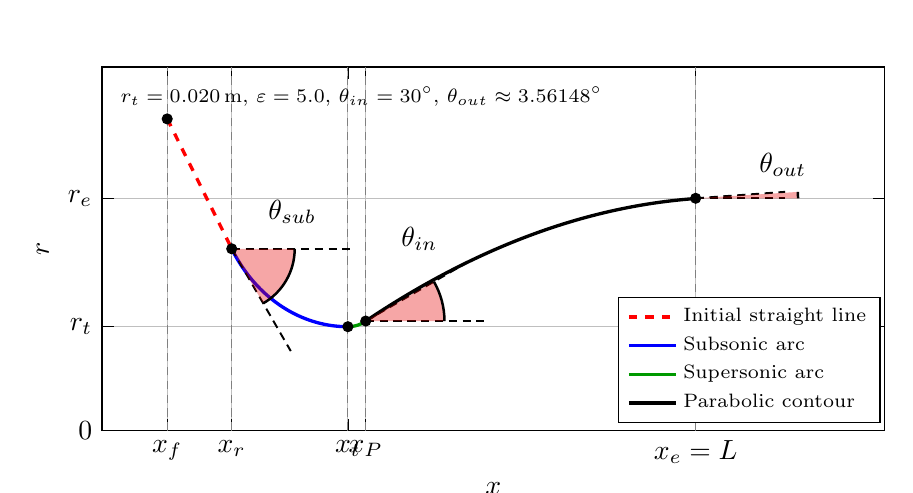
\begin{tikzpicture}
\begin{axis}[
    width=0.95\linewidth,
    height=6.2cm,
    grid=both,
    xlabel={$x$},
    ylabel={$r$},
    xmin=0, xmax=0.175,
    ymin=0, ymax=0.07,
    trig format=deg,
    scaled ticks=false,
    tick style={black},
    legend style={at={(0.995,0.02)},anchor=south east,fill=white,draw=black,line width=0.4pt,font=\scriptsize},
    legend cell align=left,
]

\pgfmathsetmacro{\rt}{0.020}
\pgfmathsetmacro{\eps}{5.0}
\pgfmathsetmacro{\re}{sqrt(\eps)*\rt}
\pgfmathsetmacro{\alphaDeg}{15}
\pgfmathsetmacro{\bell}{0.80}
\pgfmathsetmacro{\thetaSubDeg}{60}
\pgfmathsetmacro{\thetaInDeg}{30}
\pgfmathsetmacro{\Rch}{0.060}
\pgfmathsetmacro{\tx}{0.055}

\pgfmathsetmacro{\xr}{-1.5*\rt*sin(\thetaSubDeg)}
\pgfmathsetmacro{\yr}{2.5*\rt - 1.5*\rt*cos(\thetaSubDeg)}
\pgfmathsetmacro{\xR}{\tx+\xr}
\pgfmathsetmacro{\mLine}{-tan(\thetaSubDeg)}
\pgfmathsetmacro{\bLine}{\yr - \mLine*\xr}
\pgfmathsetmacro{\xf}{(\Rch - \bLine)/\mLine}
\pgfmathsetmacro{\xF}{\tx+\xf}

\pgfmathsetmacro{\rSup}{0.4*\rt}
\pgfmathsetmacro{\Px}{\rSup*sin(\thetaInDeg)}
\pgfmathsetmacro{\Py}{1.4*\rt - \rSup*cos(\thetaInDeg)}
\pgfmathsetmacro{\xP}{\tx+\Px}

\pgfmathsetmacro{\Lcone}{(\re-\rt)/tan(\alphaDeg)}
\pgfmathsetmacro{\L}{\Px + \bell*\Lcone}
\pgfmathsetmacro{\xE}{\tx+\L}
\pgfmathsetmacro{\mZero}{tan(\thetaInDeg)}
\pgfmathsetmacro{\den}{(\L-\Px)}
\pgfmathsetmacro{\aPar}{(\re - \Py - \mZero*(\den))/(\den*\den)}
\pgfmathsetmacro{\bPar}{\mZero - 2*\aPar*\Px}
\pgfmathsetmacro{\cPar}{\Py - \aPar*\Px*\Px - \bPar*\Px}
\pgfmathsetmacro{\thetaOutDeg}{atan(2*\aPar*\L + \bPar)}
\pgfmathsetmacro{\mOut}{tan(\thetaOutDeg)}

\pgfplotsset{
  xtick={\xF,\xR,\tx,\xP,\xE},
  xticklabels={$x_f$,$x_r$,$x_t$,$x_P$,$x_e=L$},
  ytick={0,\rt,\re},
  yticklabels={$0$,$r_t$,$r_e$},
}

\addplot[dashed, very thick, red, domain=\xF:\xR, samples=2] ({x},{\mLine*(x-\tx)+\bLine});
\addlegendentry{Initial straight line}

\addplot[very thick, blue, domain=\xR:\tx, samples=250] ({x},{2.5*\rt - sqrt((1.5*\rt)^2 - (x-\tx)^2)});
\addlegendentry{Subsonic arc}

\addplot[very thick, green!60!black, domain=\tx:\xP, samples=250] ({x},{1.4*\rt - sqrt((0.4*\rt)^2 - (x-\tx)^2)});
\addlegendentry{Supersonic arc}

\addplot[very thick, black, domain=\xP:\xE, samples=350] ({x},{\aPar*(x-\tx)^2 + \bPar*(x-\tx) + \cPar});
\addlegendentry{Parabolic contour}

\addplot[only marks, mark=*, mark size=1.8pt] coordinates {(\xF,\Rch) (\xR,\yr) (\tx,\rt) (\xP,\Py) (\xE,\re)};

\addplot[densely dashed, gray] coordinates {(\xF,0) (\xF,0.07)};
\addplot[densely dashed, gray] coordinates {(\xR,0) (\xR,0.07)};
\addplot[densely dashed, gray] coordinates {(\tx,0) (\tx,0.07)};
\addplot[densely dashed, gray] coordinates {(\xP,0) (\xP,0.07)};
\addplot[densely dashed, gray] coordinates {(\xE,0) (\xE,0.07)};

\path (axis cs:\xR,\yr) coordinate (Rpt);
\path (axis cs:\xP,\Py) coordinate (Ppt);
\path (axis cs:\xE,\re) coordinate (Ept);

\tikzset{angline/.style={densely dashed, black, line width=0.7pt}}

\def\Lsub{15mm}
\def\RadFillSub{8mm}
\def\RadArcSub{8mm}
\pgfmathsetmacro{\phiSub}{\thetaSubDeg}
\draw[angline] (Rpt) -- ++(\Lsub,0);
\draw[angline] (Rpt) -- ++(-\phiSub:\Lsub);
\fill[red!90!black, opacity=0.35] (Rpt) -- ++(\RadFillSub,0) arc[start angle=0, end angle=-\phiSub, radius=\RadFillSub] -- cycle;
\draw[black, line width=0.9pt] (Rpt) ++(\RadArcSub,0) arc[start angle=0, end angle=-\phiSub, radius=\RadArcSub];
\node[anchor=south west] at (axis cs:\xR+0.006,\yr+0.003) {$\theta_{sub}$};

\def\Lin{15mm}
\def\RadFillIn{10mm}
\def\RadArcIn{10mm}
\pgfmathsetmacro{\phiIn}{\thetaInDeg}
\draw[angline] (Ppt) -- ++(\Lin,0);
\draw[angline] (Ppt) -- ++(\phiIn:\Lin);
\fill[red!90!black, opacity=0.35] (Ppt) -- ++(\RadFillIn,0) arc[start angle=0, end angle=\phiIn, radius=\RadFillIn] -- cycle;
\draw[black, line width=0.9pt] (Ppt) ++(\RadArcIn,0) arc[start angle=0, end angle=\phiIn, radius=\RadArcIn];
\node[anchor=north] at (axis cs:\xP+0.012,\Py+0.02) {$\theta_{in}$};

\pgfmathsetmacro{\dxE}{0.020}
\draw[angline] (axis cs:\xE,\re) -- (axis cs:\xE+\dxE,\re);
\pgfmathsetmacro{\dyE}{\mOut*\dxE}
\draw[angline] (axis cs:\xE,\re) -- (axis cs:\xE+\dxE,\re+\dyE);
\pgfmathsetmacro{\phiOut}{\thetaOutDeg}
\def\RadFill{13mm}
\def\RadArc{13mm}
\path (Ept) ++(\RadFill,0) coordinate (FillStart);
\fill[red!90!black, opacity=0.35] (Ept) -- (FillStart) arc[start angle=0, end angle=\phiOut, radius=\RadFill] -- cycle;
\path (Ept) ++(\RadArc,0) coordinate (ArcStart);
\draw[black, line width=0.9pt] (ArcStart) arc[start angle=0, end angle=\phiOut, radius=\RadArc];
\node[anchor=center] at (rel axis cs:0.87,0.73) {$\theta_{out}$};

\node[anchor=north west] at (axis cs:0.002,0.068) {\scriptsize $r_t=\rt\,\mathrm{m}$, $\varepsilon=\eps$, $\theta_{in}=\thetaInDeg^\circ$, $\theta_{out}\approx\thetaOutDeg^\circ$};

\end{axis}
\end{tikzpicture}
\caption{Two-dimensional nozzle contour with region definitions, stations and angle notation.}
\label{fig:nozzle_piecewise_tikz}
\end{figure}

% =========================================================
\section{Numerical Coordinate Conditioning and Two-Dimensional Contour Output}
% =========================================================

\subsection{Translated contour representation and plotting quantities}

\subsubsection{Axial coordinate translation}

The throat-centered coordinate system is convenient for mathematical construction, but it produces negative $x$ values in the subsonic converging section. For plotting, CAD export and easier interpretation, the profile is translated horizontally so that the first point of the nozzle starts at $x=0$.

The required translation is
\begin{equation}
\Delta x=-x_f.
\label{eq:translation_simple}
\end{equation}

Using the line geometry, this can also be written as
\begin{equation}
\Delta x=-x_r+\frac{r_c-r_r}{\tan(\theta_{sub})}.
\label{eq:translation}
\end{equation}

After translation, all axial coordinates become
\begin{equation}
\bar{x}=x+\Delta x.
\end{equation}

The translated domain is
\begin{equation}
\bar{x}\in[0,L-x_f].
\end{equation}

\begin{figure}[H]
    \centering
    \IfFileExists{cad3.png}{
\includegraphics[width=0.75\linewidth]{cad3.png}}{\fbox{\parbox{0.75\linewidth}{\centering Missing figure file: \texttt{cad3.png}}}}
    \caption{Horizontal translation used to move the nozzle start to $x=0$.}
    \label{fig:translation}
\end{figure}

\subsubsection{Derived geometric outputs}

The simulator outputs several secondary quantities that help evaluate the geometry:
\begin{align}
CR &= \frac{r_c^2}{r_t^2},\\
\varepsilon &= \frac{r_e^2}{r_t^2},\\
L_{nozzle} &= L-x_f,\\
\theta_{out} &= \arctan(2aL+b).
\end{align}

These quantities are displayed together with the two-dimensional profile to make each generated geometry immediately interpretable.

\begin{figure}[H]
    \centering
    \IfFileExists{plot2D.png}{
\includegraphics[width=0.78\linewidth]{plot2D.png}}{\fbox{\parbox{0.78\linewidth}{\centering Missing figure file: \texttt{plot2D.png}}}}
    \caption{Example of a generated two-dimensional nozzle geometry profile.}
    \label{fig:plot2D}
\end{figure}

\begin{figure}[H]
    \centering
    \begin{subfigure}{0.48\linewidth}
        \centering
        \IfFileExists{ex2.png}{
\includegraphics[width=\linewidth]{ex2.png}}{\fbox{\parbox{0.95\linewidth}{\centering Missing: \texttt{ex2.png}}}}
        \caption{First geometry example.}
    \end{subfigure}
    \hfill
    \begin{subfigure}{0.48\linewidth}
        \centering
        \IfFileExists{ex3.png}{
\includegraphics[width=\linewidth]{ex3.png}}{\fbox{\parbox{0.95\linewidth}{\centering Missing: \texttt{ex3.png}}}}
        \caption{Second geometry example.}
    \end{subfigure}
    \caption{Example two-dimensional outputs generated from different input parameters.}
    \label{fig:2D_examples}
\end{figure}

% =========================================================
\section{Axisymmetric Three-Dimensional Geometry Reconstruction}
% =========================================================

\subsection{Revolution-based surface generation}

\subsubsection{Surface-of-revolution definition}

Because the nozzle is axisymmetric, the three-dimensional surface is generated by revolving the two-dimensional radius function around the nozzle axis. For each axial coordinate $x_i$ and radius $r_i$, a circular ring is generated using the angular coordinate $\phi$:
\begin{align}
X_i(\phi)&=x_i,\\
Y_i(\phi)&=r_i\cos\phi,\\
Z_i(\phi)&=r_i\sin\phi,
\end{align}
with
\begin{equation}
\phi\in[0,2\pi].
\end{equation}

The complete nozzle surface is therefore
\begin{equation}
\bm{S}(x,\phi)=
\begin{bmatrix}
x\\
r(x)\cos\phi\\
r(x)\sin\phi
\end{bmatrix}.
\label{eq:surface_of_revolution}
\end{equation}

This formulation is important because it makes clear that the three-dimensional geometry is not an independent model. It is the direct revolution of the piecewise two-dimensional contour from Eq.~\eqref{eq:piecewise_nozzle}.

\subsubsection{Structured mesh matrices for visualization}

For numerical visualization, the axial and angular coordinates are assembled into matrices. If
\begin{equation}
\bm{x}=\begin{bmatrix}x_0&x_1&\cdots&x_n\end{bmatrix}^T,
\end{equation}
and
\begin{equation}
\bm{\phi}=\begin{bmatrix}\phi_0&\phi_1&\cdots&\phi_m\end{bmatrix},
\end{equation}
then the axial mesh has the structure
\begin{equation}
X=\begin{bmatrix}
x_0&x_0&\cdots&x_0\\
x_1&x_1&\cdots&x_1\\
\vdots&\vdots&\ddots&\vdots\\
x_n&x_n&\cdots&x_n
\end{bmatrix}.
\label{eq:Xmesh}
\end{equation}

The angular mesh is
\begin{equation}
\Phi=\begin{bmatrix}
\phi_0&\phi_1&\cdots&\phi_m\\
\phi_0&\phi_1&\cdots&\phi_m\\
\vdots&\vdots&\ddots&\vdots\\
\phi_0&\phi_1&\cdots&\phi_m
\end{bmatrix}.
\label{eq:Phimesh}
\end{equation}

The radial mesh is
\begin{equation}
R=\begin{bmatrix}
r_0&r_0&\cdots&r_0\\
r_1&r_1&\cdots&r_1\\
\vdots&\vdots&\ddots&\vdots\\
r_n&r_n&\cdots&r_n
\end{bmatrix}.
\label{eq:Rmesh}
\end{equation}

The Cartesian surface matrices are finally
\begin{align}
Y &= R\cos\Phi,\\
Z &= R\sin\Phi.
\end{align}

\subsubsection{Three-dimensional geometry inspection}

The three-dimensional plot is used as a quick visual validation before exporting the profile to CAD. It helps identify discontinuities, wrong radius values, exaggerated exit radii, incorrect translations or malformed parabolic contours.

\begin{figure}[H]
    \centering
    \IfFileExists{ex4.png}{
\includegraphics[width=0.88\linewidth]{ex4.png}}{\fbox{\parbox{0.88\linewidth}{\centering Missing figure file: \texttt{ex4.png}}}}
    \caption{Example of three-dimensional nozzle visualization generated by surface revolution.}
    \label{fig:3D_view}
\end{figure}

\begin{figure}[H]
    \centering
    \IfFileExists{ex10.png}{
\includegraphics[width=0.88\linewidth]{ex10.png}}{\fbox{\parbox{0.88\linewidth}{\centering Missing figure file: \texttt{ex10.png}}}}
    \caption{Example of multi-view visualization of the generated nozzle geometry.}
    \label{fig:3D_multiview}
\end{figure}

% =========================================================
\section{CAD-Oriented Geometry Export and Manufacturing Workflow}
% =========================================================

\subsection{Point-cloud conditioning and CAD reconstruction}

\subsubsection{CAD-compatible coordinate export}

One of the main practical objectives of the simulator is to export the generated contour to a CAD-compatible point file. The exported coordinates represent the two-dimensional meridional profile of the nozzle and can be imported into software such as Autodesk Fusion or SolidWorks.

The exported point set has the form
\begin{equation}
\mathcal{P}=\left\{(x_i,r_i,0)\right\}_{i=0}^{N}.
\end{equation}

The third coordinate is set to zero because the imported curve is a planar sketch. The three-dimensional nozzle body is then obtained in CAD by offsetting the wall thickness and revolving the profile around the nozzle axis.

\subsubsection{Point filtering and sketch-conditioning strategy}

A very dense point set is useful for smooth numerical plots, but it can overdefine a CAD sketch. Excessive point density may cause spline irregularities, local oscillations or unstable sketch constraints. Therefore, the CAD export uses fewer points than the plotting routine.

The point selection follows two principles:
\begin{enumerate}
    \item preserve all important geometric regions, including the subsonic arc, throat, supersonic arc and parabolic contour;
    \item impose a minimum spacing between consecutive exported points to avoid point clustering.
\end{enumerate}

This produces a smoother and more robust CAD sketch while maintaining the essential contour shape.

\begin{figure}[H]
    \centering
    \begin{subfigure}{0.48\linewidth}
        \centering
        \IfFileExists{ex11.png}{
\includegraphics[width=\linewidth]{ex11.png}}{\fbox{\parbox{0.95\linewidth}{\centering Missing: \texttt{ex11.png}}}}
        \caption{Overdefined sketch irregularity.}
    \end{subfigure}
    \hfill
    \begin{subfigure}{0.48\linewidth}
        \centering
        \IfFileExists{ex12.png}{
\includegraphics[width=\linewidth]{ex12.png}}{\fbox{\parbox{0.95\linewidth}{\centering Missing: \texttt{ex12.png}}}}
        \caption{Close view near throat transition.}
    \end{subfigure}
    \caption{CAD sketch irregularities caused by unsuitable point distribution.}
    \label{fig:cad_irregularity}
\end{figure}

\subsubsection{CAD reconstruction workflow}

The practical workflow is:
\begin{enumerate}
    \item generate the two-dimensional contour using the geometric model;
    \item translate the axial coordinates so that the first point starts at zero;
    \item reduce and filter the point set for CAD stability;
    \item export the coordinates in millimetres;
    \item import the point file into CAD;
    \item create a spline through the imported points;
    \item offset the contour to define wall thickness;
    \item revolve the final closed sketch around the nozzle axis.
\end{enumerate}

\begin{figure}[H]
    \centering
    \IfFileExists{ex13.png}{
\includegraphics[width=0.85\linewidth]{ex13.png}}{\fbox{\parbox{0.85\linewidth}{\centering Missing figure file: \texttt{ex13.png}}}}
    \caption{Example of exported nozzle coordinates opened as a table.}
    \label{fig:csv_output}
\end{figure}

\begin{figure}[H]
    \centering
    \IfFileExists{ex14.png}{
\includegraphics[width=0.82\linewidth]{ex14.png}}{\fbox{\parbox{0.82\linewidth}{\centering Missing figure file: \texttt{ex14.png}}}}
    \caption{Imported contour sketch in CAD after point reduction and filtering.}
    \label{fig:cad_sketch}
\end{figure}

\begin{figure}[H]
    \centering
    \begin{subfigure}{0.48\linewidth}
        \centering
        \IfFileExists{ex16.png}{
\includegraphics[width=\linewidth]{ex16.png}}{\fbox{\parbox{0.95\linewidth}{\centering Missing: \texttt{ex16.png}}}}
        \caption{Wall-thickness offset.}
    \end{subfigure}
    \hfill
    \begin{subfigure}{0.48\linewidth}
        \centering
        \IfFileExists{ex17.png}{
\includegraphics[width=\linewidth]{ex17.png}}{\fbox{\parbox{0.95\linewidth}{\centering Missing: \texttt{ex17.png}}}}
        \caption{Final revolved nozzle body.}
    \end{subfigure}
    \caption{CAD operations used to convert the generated contour into a manufacturable three-dimensional body.}
    \label{fig:cad_final}
\end{figure}



% =========================================================
\section{Genetic-Algorithm Optimization Framework}
% =========================================================

\subsection{Optimization problem definition}

\subsubsection{Chromosome definition and design variables}

The geometric formulation can be used directly inside a genetic algorithm. A candidate nozzle geometry may be represented by the chromosome
\begin{equation}
\bm{q}=\begin{bmatrix}
r_t & \varepsilon & \theta_{sub} & \theta_{in} & \alpha & K_b & r_c
\end{bmatrix}^T.
\label{eq:chromosome}
\end{equation}

Depending on the design problem, some variables may be fixed. For example, if the engine mass flow rate and chamber pressure already define the throat radius, then $r_t$ should be fixed by Eq.~\eqref{eq:throat_radius} and should not be freely optimized. Similarly, $r_c$ may be constrained by the combustion chamber geometry.

A practical optimization vector may therefore be reduced to
\begin{equation}
\bm{q}_{opt}=\begin{bmatrix}
\varepsilon & \theta_{in} & K_b
\end{bmatrix}^T,
\label{eq:chromosome_reduced}
\end{equation}
while $r_t$, $r_c$, $\theta_{sub}$ and $\alpha$ remain prescribed by engine sizing or design rules.

\subsubsection{Geometric and physical constraint handling}

The genetic algorithm must reject or penalize geometries that violate physical or manufacturing constraints. Typical constraints include:
\begin{align}
r_t &>0,\\
r_e &=\sqrt{\varepsilon}r_t>r_t,\\
CR &=\frac{r_c^2}{r_t^2}>1,\\
L_{nozzle} &\leq L_{max},\\
\theta_{out} &\leq \theta_{out,max},\\
r_{eff}(x)&>0 \quad \forall x,\\
\kappa(x)&\leq \kappa_{max} \quad \text{if a curvature limit is imposed.}
\end{align}

These constraints prevent the optimizer from producing mathematically valid but physically unusable contours.

\subsubsection{Fitness-function definition}

A simple objective function can maximize corrected specific impulse:
\begin{equation}
J(\bm{q})=I_{sp,ideal}(\bm{q})\eta_{total}(\bm{q}).
\label{eq:objective_Isp}
\end{equation}

Equivalently, the algorithm may minimize the negative objective:
\begin{equation}
\min_{\bm{q}}\left[-I_{sp,ideal}(\bm{q})\eta_{total}(\bm{q})\right].
\end{equation}

A more complete multi-penalty objective can include length, overexpansion risk and manufacturability:
\begin{equation}
J(\bm{q})=I_{sp,ideal}\eta_{total}
-w_L\frac{L_{nozzle}}{L_{ref}}
-w_p\left|\frac{p_e-p_a}{p_a}\right|
-w_c\frac{\Phi_s}{\Phi_{ref}},
\label{eq:objective_full}
\end{equation}
where $w_L$, $w_p$ and $w_c$ are weighting coefficients.

\subsubsection{Engineering interpretation of optimized geometries}

The main advantage of this formulation is interpretability. If the optimizer increases $\varepsilon$, the reason is usually improved expansion and exit velocity. If it reduces $\theta_{out}$, the reason is lower divergence loss. If it increases the bell length fraction $K_b$, the reason may be smoother turning and lower curvature penalty. If it reduces $\theta_{in}$, the reason may be lower early supersonic turning severity.

Therefore, the genetic algorithm should not be treated as a black box. Its final geometry should be analyzed through the same quantities used to construct the model: $r(x)$, $M(x)$, $p(x)$, $T(x)$, $\theta_{out}$, $\eta_{div}$, $\eta_{BL}$, $\eta_{turn}$ and $\eta_{total}$.

% =========================================================
\section{Results and Discussion}
% =========================================================

\subsection{Simulator outputs and engineering interpretation}

\subsubsection{Piecewise-contour generation}

The simulator successfully generates continuous bell nozzle profiles from a small set of input parameters. The use of circular arcs near the throat ensures smooth radius evolution through the sonic region, while the parabolic section provides a compact diverging contour with an automatically calculated exit angle.

The most important result of the geometry module is not merely the plot, but the analytical construction of Eq.~\eqref{eq:piecewise_nozzle}. This function provides a direct bridge between user inputs, flow area, Mach number calculation, three-dimensional visualization and CAD export.

\subsubsection{Axisymmetric geometry preview}

The three-dimensional preview confirms the axisymmetric interpretation of the profile and allows rapid inspection of the final geometry before CAD export. This is useful because numerical plots can hide practical problems such as excessive exit radius, poor length-to-radius proportions or local contour discontinuities.

\subsubsection{Transition from numerical contour to CAD model}

The CAD export demonstrated that point density must be managed carefully. A dense numerical contour may be excellent for plotting but poor for sketch generation. The filtered point set provides a better compromise between geometric fidelity and CAD robustness.

\subsubsection{Ideal-flow performance trends}

The ideal performance analysis provides first-order trends for exhaust velocity, temperature, ideal expansion ratio and performance parameters. These trends are useful for preliminary design but should not be interpreted as final engine predictions. They are based on isentropic assumptions and simplified thermochemical treatment.

\subsubsection{Role of correction factors in optimization}

The transition from a geometry simulator to a genetic optimizer requires additional loss modeling. Without geometric and viscous penalties, an optimizer may converge toward unrealistic geometries that exploit the ideal equations. The proposed efficiency factors provide a first physically meaningful correction layer.

% =========================================================
\section{Limitations and Future Work}
% =========================================================

The main limitations of the current formulation are:
\begin{itemize}
    \item no method-of-characteristics contour optimization;
    \item no CFD-resolved shock, separation or boundary-layer solution;
    \item no finite-rate chemistry or frozen/equilibrium transition analysis along the nozzle;
    \item simplified constant-$\gamma$ treatment in the analytical flow model;
    \item simplified turbulent displacement-thickness correlation;
    \item no thermal or structural coupling;
    \item no experimental calibration yet included in the efficiency coefficients.
\end{itemize}

Future work should include:
\begin{enumerate}
    \item integration of the genetic algorithm with the geometric model;
    \item calibration of $\eta_{div}$, $\eta_{BL}$ and $\eta_{turn}$ against CFD or experimental data;
    \item trajectory-weighted expansion-ratio selection;
    \item thermal and structural checks for manufacturable nozzle designs;
    \item direct export of smooth splines instead of only point clouds;
    \item comparison between conical, Rao-like bell and optimized bell contours.
\end{enumerate}

% =========================================================
\section{Conclusion}
% =========================================================

This work reorganizes the formulation of a single bell nozzle geometry and analysis simulator into a coherent engineering framework. The simulator constructs a complete nozzle contour from a reduced set of geometric inputs, using a straight converging line, a subsonic circular arc, a supersonic circular arc and a parabolic diverging section. The resulting piecewise function provides the basis for two-dimensional plotting, three-dimensional visualization, CAD export and quasi-one-dimensional flow analysis.

The ideal flow model uses classical isentropic relations and the area--Mach equation to determine Mach number, pressure, temperature and velocity distributions along the nozzle. Throat sizing is obtained from the choked-flow mass-flow relation, while the exit radius follows directly from the expansion ratio.

For future optimization, the ideal model is extended with physically motivated efficiency factors accounting for exit divergence, boundary-layer blockage and curvature-based turning losses. These terms allow the geometry to be mapped into corrected performance metrics suitable for genetic algorithm optimization.

The final framework is therefore not only a geometry generator, but also a foundation for automated nozzle design, where each geometric parameter has a clear mathematical and physical influence on the predicted performance.

% =========================================================
\appendix
\section{Recommended Figure Selection}

The following figures are recommended for the final article:
\begin{itemize}
    \item \texttt{image.png}: simulator functionality interface;
    \item \texttt{RPE.png} or \texttt{RPE (1).png}: reference Sutton/Biblarz bell nozzle geometry;
    \item \texttt{autocad1.png}: subsonic geometry derivation;
    \item \texttt{SupCad.png}: supersonic arc and parabola geometry derivation;
    \item TikZ plot in Fig.~\ref{fig:nozzle_piecewise_tikz}: clean final notation figure for stations and angles;
    \item \texttt{plot2D.png}, \texttt{ex2.png}, \texttt{ex3.png}: two-dimensional output examples;
    \item \texttt{ex4.png}: three-dimensional visualization;
    \item \texttt{ex11.png}, \texttt{ex12.png}: CAD point-density problem;
    \item \texttt{ex14.png}, \texttt{ex16.png}, \texttt{ex17.png}: CAD transition and final revolved body;
    \item \texttt{ex19.png}--\texttt{ex23.png}: ideal expansion and performance outputs, if the plots are visually clean.
\end{itemize}

Figures showing software installation, Python libraries, raw buttons without technical value, or repeated input windows should be moved to supplementary documentation or removed from the final article.

\begin{thebibliography}{9}

\bibitem{SuttonBiblarz}
G. P. Sutton and O. Biblarz, \textit{Rocket Propulsion Elements}, 9th ed., Wiley, 2017.

\bibitem{NASA_CEA}
S. Gordon and B. J. McBride, \textit{Computer Program for Calculation of Complex Chemical Equilibrium Compositions and Applications}, NASA Reference Publication 1311, 1994.

\bibitem{RocketCEA}
C. E. DeLong, \textit{RocketCEA Documentation}, Python interface for NASA CEA.

\bibitem{Anderson}
J. D. Anderson, \textit{Modern Compressible Flow: With Historical Perspective}, McGraw-Hill.

\end{thebibliography}

\end{document}
% ARCHIVED SOURCE SNAPSHOT -- retained to preserve the original ZIP structure.
% The synchronized, publication-ready build entry point is main.tex.
